%%%%%%%%%%%%%%%%%%%%%%%%%%%%%%%%%%%%%%%%
%% MCM/ICM LaTeX Template %%
%% 2022 MCM/ICM           %%
%%%%%%%%%%%%%%%%%%%%%%%%%%%%%%%%%%%%%%%%
\documentclass[12pt]{article}
\usepackage{geometry}
\geometry{left=1in,right=0.75in,top=1in,bottom=1in}

%%%%%%%%%%%%%%%%%%%%%%%%%%%%%%%%%%%%%%%%
% Replace ABCDEF in the next line with your chosen problem
% and replace 1111111 with your Team Control Number
\newcommand{\Problem}{A}
\newcommand{\Team}{2200655}
%%%%%%%%%%%%%%%%%%%%%%%%%%%%%%%%%%%%%%%%

\usepackage{newtxtext}
\usepackage{amsmath,amssymb,amsthm}
\usepackage{newtxmath} % must come after amsXXX

\usepackage{graphicx}
\usepackage{xcolor}
\usepackage{fancyhdr}
%%%%%%%%%%%%%%%%%%%%%%%%%%%%%%%%%%%%%%%%
\usepackage{lipsum}
\usepackage{svg}
\usepackage{tabularx}
\usepackage{epstopdf}
\usepackage{mathrsfs}
\usepackage{longtable}
\usepackage{cite}
\usepackage{makecell}
\usepackage{diagbox}
\lhead{Team \Team}
\rhead{}
\cfoot{}

\newtheorem{theorem}{Theorem}
\newtheorem{corollary}[theorem]{Corollary}
\newtheorem{lemma}[theorem]{Lemma}
\newtheorem{definition}{Definition}

%%%%%%%%%%%%%%%%%%%%%%%%%%%%%%%%
\begin{document}
\graphicspath{{./figure/}{../problem/data/athletes/}}  % Place your graphic files in the same directory as \includesvgg, .svg, .eps}
\thispagestyle{empty}
\vspace*{-16ex}
\centerline{\begin{tabular}{*3{c}}
        \parbox[t]{0.3\linewidth}{\begin{center}\textbf{Problem Chosen}\\ \Large \textcolor{red}{\Problem}\end{center}}
         & \parbox[t]{0.3\linewidth}{\begin{center}\textbf{2022\\ MCM/ICM\\ Summary Sheet}\end{center}}
         & \parbox[t]{0.3\linewidth}{\begin{center}\textbf{Team Control Number}\\ \Large \textcolor{red}{\Team}\end{center}} \\
        \hline
    \end{tabular}}
%%%%%%%%%%% Begin Summary %%%%%%%%%%%
% Enter your summary here replacing the (red) text
% Replace the text from here ...
\begin{center}
    \textbf{Summary}
\end{center}
In an individual time trial, each individual
cyclist is expected to ride a fixed course alone, and the winner is the rider who does so in the
least amount of time.

Riders are always looking to minimize the time required to cover a given distance. Given a
particular rider's capability according to that rider's power curve, how should that rider apply
power while traversing a given time trial course?
Our team aims to establish a model that can give the optimal plan for any particular rider, which tells them exactly when to accelerate,
and when to slow down so that they can make the best of themselves. Firstly, we assume the air to be stationary and designed a mathematical model of movement
in the race, and then we studied the power-duration models built by multiple articles(Mark Burnley \& Andrew M. Jones, 2016)\cite{doi:10.1080/17461391.2016.1249524}
(Peter Leo,2021)\cite{leo2021power}(Andrea Zignoli, Francesco Biral,2020)\cite{zignoli2020prediction}, and found that all of them can be described as the product of time and the difference
between the power in this period and the critical power $CP$ is a constant value, which we denote as $R_0$ ,thus we can  set restrictions  to simulate how fatigue
will influence the riders in a race.

In reality, the rider have to focus on the riding, they can not change their power all the time, thus building a continuous model is not only very complex,
but also unnecessary and unless. So we think it is only reasonable that we discretize the time in a race  it and use dynamic programming to analyze the power strategy in each
period and find the best solution, and a proof of the reasonableness of this method will be given later.

Then we are going to test our model on serval riders in a given TT(time trial) race. We need them to be various, we shall choose two different types of rider, time trial
specialists and climbers, and we will define a male and a female for each of the two types of riders. To keep the data from getting out of line, we analyze the power curve
from https://www.strava.com/pros following the following steps:
First, we derive from our model that the equation of the curve should be exponential, which is $y=m*n^x+k$, and it fits the curve we acquired.
Then we fit all four riders' power curve to the equation, we get the value of $m,n,k$ for each rider. Accounting to our model, we found the relationship between these
coefficients and our parameters and built the power profile of them.

We also need the map of the race, we found the course profile from https://www.flanders2021.com
then use the Reverse-Engineering Visualizations method developed by Jorge Poco1 and Jeffrey Heer in 2017\cite{poco2017reverse} to get the data we need about the racing track.

Next, based on the above models, we are able to test model. What's more, we improved our model. First by taking the weather into account, we mainly analyze the influence of the
wind, for the air friction is the main resistance, in stronger wind, which the speed of wind is fast, thus the air friction will be huge accounting to the equation of the
equation of air friction, and the riders' speed will drop considerably.

Finally, we are able to  give a two-page detailed guide to the riders and their team.
\begin{center}
    \textbf{Keywords:}\Large Dynamic Programming, Power-duration model, Discretization

\end{center}
\textbf{Follow us @COMAPMath on Twitter or COMAPCHINAOFFICIAL on Weibo for the \newline
    most up to date contest information.}


% to here
%%%%%%%%%%% End Summary %%%%%%%%%%%

%%%%%%%%%%%%%%%%%%%%%%%%%%%%%%
\clearpage
\pagestyle{fancy}
% Uncomment the next line to generate a Table of Contents
%\tableofcontents 
\newpage
\setcounter{page}{1}
\rhead{Page \thepage\ }
%%%%%%%%%%%%%%%%%%%%%%%%%%%%%%
\title{Storing the Sun:a Model for Off-grid Power System Design}
\Large
\maketitle
\tableofcontents   % 若不想要目录, 注释掉该句
\newpage
%%%%%%%%%%%%%%%%%%%%%%%%%%%%%%%%%%%%%%%%%%%%%%%%%%
\section{Introduction}
\subsection{Background}

There are many types of bicycle road races including a criterium, a team time trial, and an
individual time trial. A rider's chance of success can vary for these contests depending on the
type of event, the course, and the rider's abilities. In an individual time trial, each individual
cyclist is expected to ride a fixed course alone, and the winner is the rider who does so in the
least amount of time.

An individual rider can produce different levels of power for different lengths of time, and the
amount of power and how long a given amount of power a rider can produce varies greatly
between riders. A rider's power curve indicates how long a rider can produce a given amount of
power. In other words, for a particular length of time the power curve provides the maximum
power a rider can maintain for that given time. Generally, the more power a rider produces, the
less time the rider can maintain that power before having to reduce the amount of power and
recover. A rider may choose to briefly exceed the limits on their power curve, but the rider then
requires extra time at a lower power level to recover. Moreover, a rider's power output in the
past matters, and riders are increasingly fatigued as a race progresses.

Riders are always looking to minimize the time required to cover a given distance. Given a
particular rider's capability according to that rider's power curve, how should that rider apply
power while traversing a given time trial course? Additionally, many types of riders may
participate in an individual time trial, such as a time trial specialist, a climber, a sprinter, a
rouleur, or a puncheur, and each type of rider has a distinct power curve.

Our team aims to establish a model that can give the optimal plan for any particular rider, which tells them exactly when to accelerate,
and when to slow down so that they can make the best of themselves.
\subsection{Restatement of the Problem}
Our team aims to establish a model that can give the optimal plan for any particular rider, which tells them exactly when to accelerate,
and when to slow down so that they can make the best of themselves. Firstly, we assume the air to be stationary and designed a mathematical model of movement
in the race, we shall also try to find a power-duration model that is supported by repeatable experiences thus we can  set restrictions  to simulate how fatigue
will influence the riders in a race.
\subsubsection{Requirement 1}
First we shall define a few "volunteers" to test our model, we need them to be various, we shall choose two different types of rider, time trial
specialists and climbers, and we will define a male and a female for each of the two types of riders. To keep the data from getting out of line, we will analyze the data of
real pro riders. We should first find the source of that data and find a way to get the parameters we need in our model
\subsubsection{Requirement 2}


\subsubsection{Requirement 3}

\subsubsection{Requirement 4}

\subsection{Requirement 5}

\subsection{Requireemt 6}

\section{Assumptions and Justification}

To simplify the problem and make it convenient for us to simulate real-life conditions, we make the following basic assumptions, each of which is properly justified.

\begin{itemize}
    \item {\bf The change of speed is instant}

\end{itemize}
\section{Notations}
\begin{center}
    \resizebox{\textwidth}{!}{
        \begin{tabular}{clc}
            {\bf Symbols} & {\bf Description}                                       & \quad {\bf Unit}  \\[0.25cm]
            $A$           & Frontal area                                            & \quad $m^2$       \\[0.25cm]
            $E$           & Stamina-to-work conversion efficiency                   & \quad $J^{-1}$    \\[0.25cm]
            $v$           & Velocity of the rider                                   & \quad $kW\cdot h$ \\[0.25cm]
            $v_m$         & Velocity of the wind                                    & \quad $kW\cdot h$ \\[0.25cm]
            $\eta $       & Transmission efficiency of the bike                     & \quad No units    \\[0.25cm]
            $\rho $       & Density of the air                                      & \quad $kg/m^3$    \\[0.25cm]
            $C_w$         & drag coefficient                                        & \quad No units    \\[0.25cm]
            $C_r$         & coefficient of rolling friction                         & \quad No units    \\[0.25cm]
            $F_r$         & Rolling friction resistance                             & \quad $N$         \\[0.25cm]
            $F_w$         & Air friction                                            & \quad $N$         \\[0.25cm]
            $F_s$         & The components of gravity in the direction of the slope & \quad $N$         \\[0.25cm]
            $f$           & Resistance                                              & \quad $N$         \\[0.25cm]
            $m$           & Number of types of lithium batteries                    & \quad No units    \\[0.25cm]
            $\theta $     & Angle of a slope                                        & \quad rad         \\[0.25cm]
            $M$           & Maximum  power of the rider                             & \quad $W$         \\[0.25cm]
            $R$           & Stamina at the moment                                   & \quad No units    \\[0.25cm]
            $CP$          & Recovery                                                & \quad $s^{-1}$    \\[0.25cm]
            $R_0$         & Maximum Stamina                                         & \quad No unit     \\[0.25cm]
            $P$           & Power of the rider                                      & \quad $W$         \\[0.25cm]
            $L$           & lactate effect                                          & \quad $W$         \\[0.25cm]
        \end{tabular}
    }
\end{center}
\section{Model Development}
We aim to make an individualized, thorough strategy for the riders, we should first find what features of them that we should take into account.
The speed of a rider
is closely related to two features, stamina(endurance), and strength. A rider that is stronger can surely ride faster--if he or she is not out of strength, and the ability
to maintain speed is called stamina.
Here we measure the strength of riders by the power of the rider riding. Research(Mark Burnley \& Andrew M. Jones, 2016)\cite{doi:10.1080/17461391.2016.1249524}
(Peter Leo,2021)\cite{leo2021power}(Andrea Zignoli, Francesco Biral,2020)\cite{zignoli2020prediction}
has showed the Power-Durance(PD) relationship
which can be described as the product of time and the difference between the power in this period and the critical power $CP$ is a constant value, which we
denote as $R_0$,  thus we can  set restrictions  to simulate how fatigue will influence our riders in a race.
\begin{equation}
    \left\{
    \begin{array}{c}
        0                \leqslant  P  \leqslant  M\frac{R}{R_0}-Lt \\
        0                \leqslant  R  \leqslant  R_0               \\
        \frac{d R}{d t}  =          Q  -          \frac{P}{E}
    \end{array}
    \right.
\end{equation}

The first restriction indicates that fatigue will slow down the rider, the lower the stamina, the less power a rider can give. The second and third restriction
showed changes of a stamina: it will slowly recover, yet it has its limit($R_0$).

Given that we aim to guide our riders, it is obvious we can not give them every detailed instructions that ask them to change their velocity continuously, so we can treat the time
as a collection of discrete time periods (here we set the length of the period to be 10s)to simplify this question and give a particle solution to guide our riders.
Then we can describe how the parameters of the rider like the distance, velocity and stamina changes in a short period of time with a set of physic equations below:
\begin{equation}
    func: \delta_p(s,p,v)=>( \delta s_p,\delta r_p,\delta v_p)=\left\{
    \begin{array}{c}
        f=F_r+F_w+F_s                   \\
        F_r=C_rmg                       \\
        F_w=\rho C_w A(v-v_w)^2         \\
        F_s=mg\sin \theta               \\
        \theta=mg\arctan\frac{d h}{d t} \\
        a=\frac{\frac{P}{v_0}-f}{m}     \\
        v_p=v_0+a                       \\
        s_p=\frac{v_0+v}{2}+s_0         \\
        s\geqslant s_0
    \end{array}
    \right.
\end{equation}

In reality, the rider have to focus on the riding, they can not change their power all the time, thus building a continuous model is not only very complex,
but also unnecessary and unless. So we split up the time in a race and use dynamic programming to find the best solution,
and a proof of the reasonableness of this method will be given later.

The state transition equation of the dynamic programming is:$$dp_{i+s_p,j+R_p,v+v_p}= min_{p = 0}^{M*\frac{j}{R}}\{dp_{i,j,v}+1\}$$

In which $i$ is the stage of time, $j$ is the stage of stamina, and $v$is the stage of velocity.
\section{Requireemt 1:Power Profile}
First we shall define a few "volunteers" to test our model, we need them to be various, we shall choose two different types of rider, time trial
specialists and climbers, and we will define a male and a female for each of the two types of riders. To keep the data from getting out of line, we analyze the power curve
from https://www.strava.com/pros following the following steps:
First, we derive from our model that if the rider keeps the maximum power that he or she can give, a term in the polynomial of the power curve,  which simulate the influence of the stamina should be exponential,
which is $m*n^x+k$, yet the influence of Lactic acid is liner, which is $l*x+k$, so the power curve should be in the form of $y=m*n^x+l*x+k$.
and it fits the curve we acquired.

\begin{figure}
    \centering
    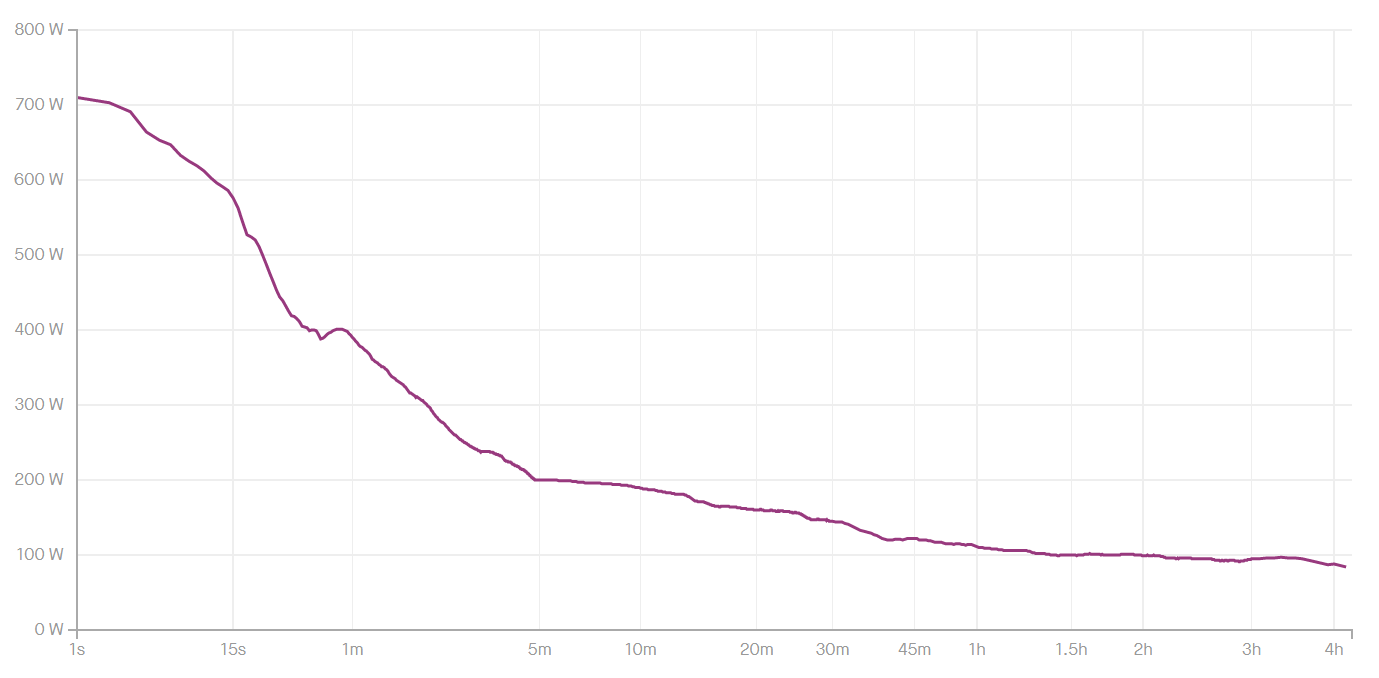
\includegraphics[width=1\columnwidth]{Eddie Anderson}
    \caption{Eddie Anderson's power curve}
\end{figure}
\begin{figure}[htbp]
    \centering
    \includesvg{Eddie Anderson}
    \caption{Eddie Anderson's fitting curve}
\end{figure}

\begin{figure}
    \centering
    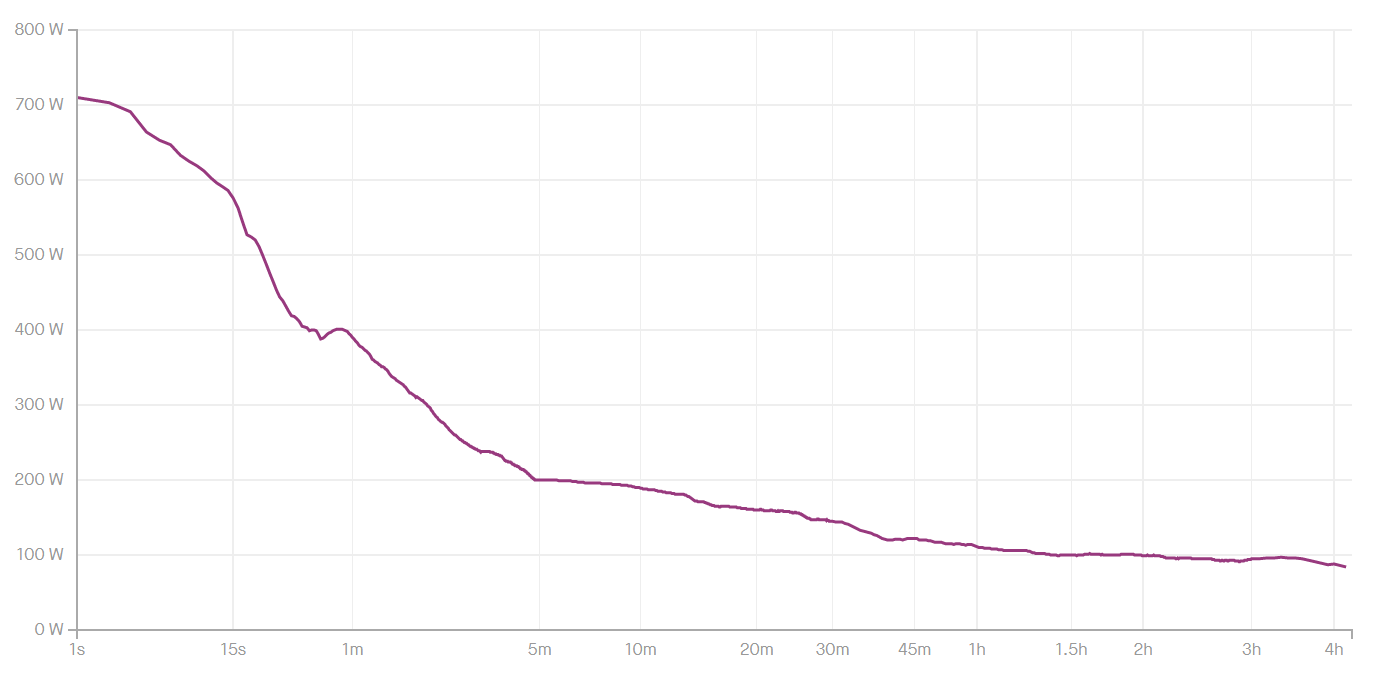
\includegraphics[width=1\columnwidth]{Jessica Allen}
    \caption{Jessica Allen's power curve}
\end{figure}
\begin{figure}
    \centering
    \includesvg{Jessica Allen}
    \caption{Jessica Allen's fitting curve}
\end{figure}

\begin{figure}
    \centering
    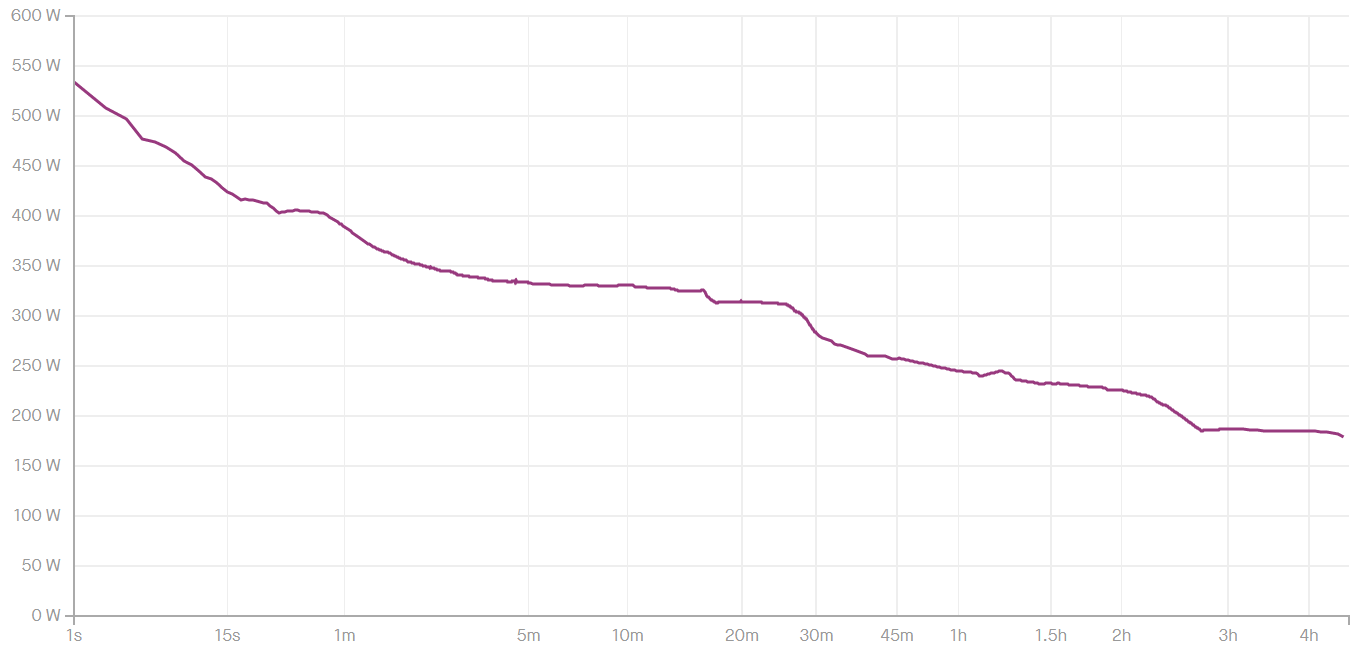
\includegraphics[width=1\columnwidth]{Johannes Weber}
    \caption{Johannes Weber's fitting curve}
\end{figure}
\begin{figure}
    \centering
    \includesvg[width=0.6\columnwidth]{Johannes Weber}
    \caption{Johannes Weber's fitting curve}
\end{figure}

\begin{figure}
    \centering
    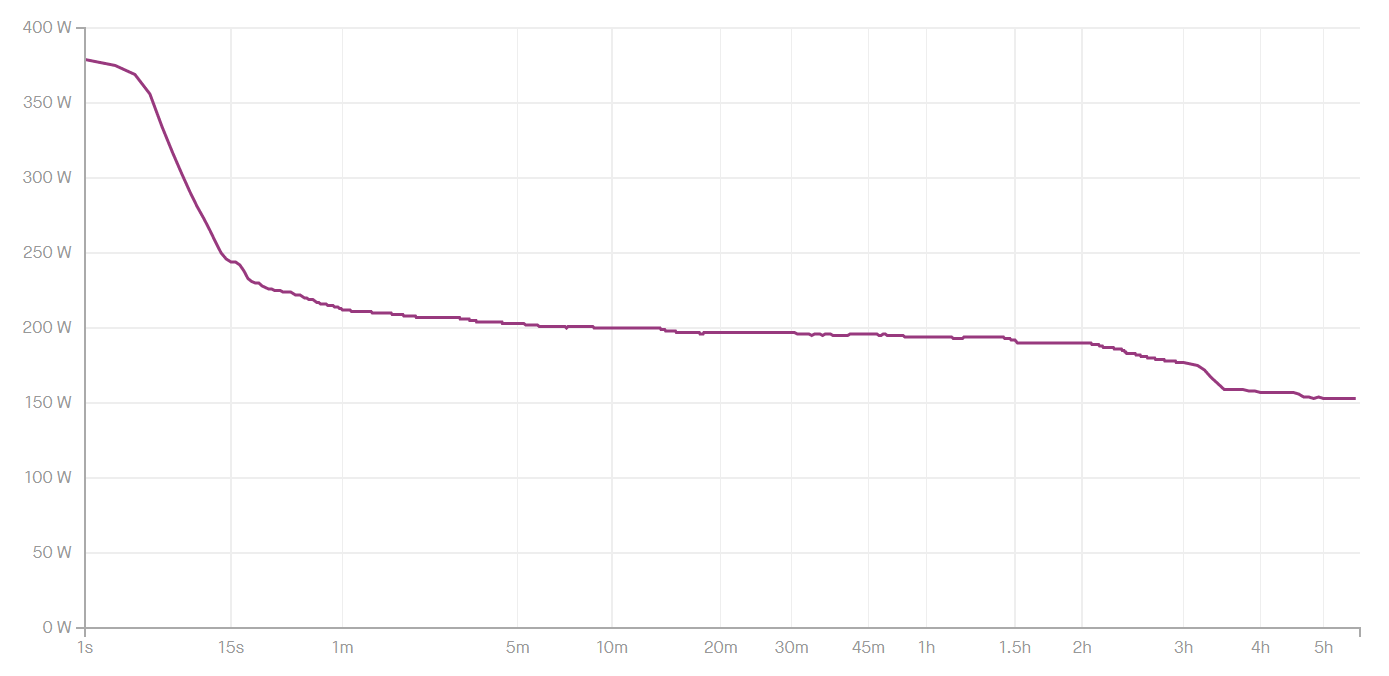
\includegraphics[width=1\columnwidth]{eackerlund}
    \caption{Erika Ackerlund's power curve}
\end{figure}
\begin{figure}
    \centering
    \includesvg{Erika Ackerlund}
    \caption{Erika Ackerlund's fitting curve}
\end{figure}
Then we fit all four riders' power curve to the equation, we get the value of $m,n,k$ for each rider. Accounting to our model, the relationship between these coefficients
and our parameters are:
\begin{equation}
    \left\{
    \begin{array}{c}
        M=n*m+k                 \\
        E=\frac{n*m+k}{R*(1-n)} \\
        CP=k*(1-n)
    \end{array}
    \right.
\end{equation}
Then, for we can set $R$ to any proper number, here we set it to 100. So we get a file of the riders.%此处应有表
Our model has the following advantages:
\begin{enumerate}
    \item The conversion efficiency and battery cost are considered together.
    \item High power electrical appliances such as hairdryers are considered, so the stability is high.
    \item The model automatically selects whether to use lithium batteries only.
    \item Constant replenishment of replaceable batteries keeps its power stable.
    \item The model can be applied to any type of battery of the same battery type.
\end{enumerate}
However, there are also some disadvantages:
\begin{enumerate}
    \item No account is taken of battery size and weight.
    \item No account is taken of different types of lithium battery life.
    \item No account is taken of the change in the number of replaceable batteries caused by different seasons
\end{enumerate}
\section{Requirement 2}
Here we will apply our model to a time trial courses--the 2021 UCI World Championship time trial course in Flanders, Belgium,--for each power profile we defined
above to prove that out model can be solved,the value of some parameter is show below:
\begin{tabular}{|c |c|}\hline
    \bf Parameters & \bf Values \\\hline
    $C_r$          & 0.003      \\\hline
    $m$            & 80         \\\hline
    $g$            & 9.8        \\\hline
    $\eta $        & 0.95       \\\hline
    $\rho  $       & 1.2        \\\hline
    $c_wA$         & 0.31       \\\hline
\end{tabular}
\begin{figure}
    \centering
    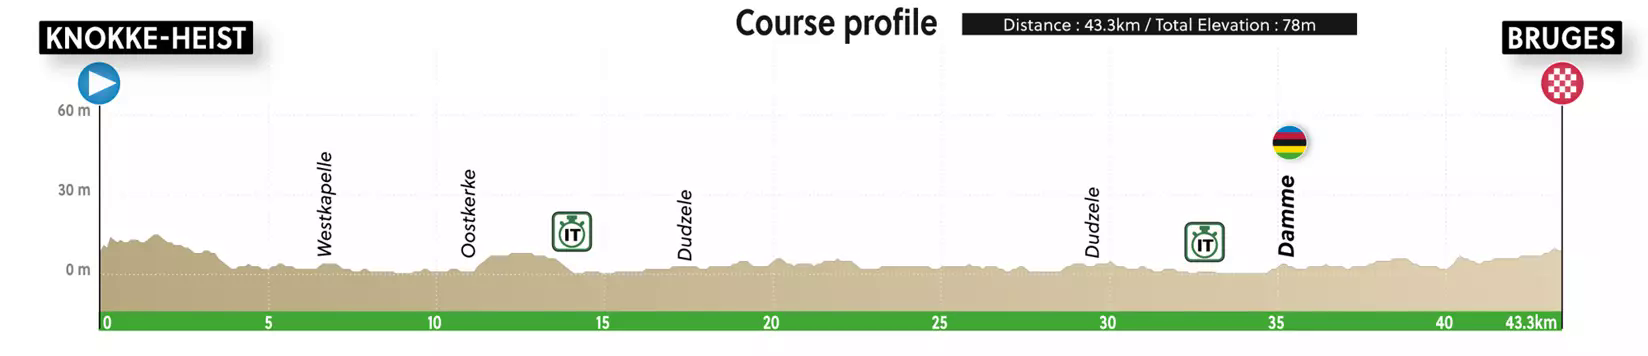
\includegraphics[width=1\columnwidth]{men-elite-individual-time-trial}
    \caption{course profile(from https://www.flanders2021.com)}
\end{figure}
We first find the course profile from https://www.flanders2021.com
then use the Reverse-Engineering Visualizations method developed by Jorge Poco1 and Jeffrey Heer in 2017\cite{poco2017reverse} to get the data we need about the racing track.
\begin{figure}
    \centering
    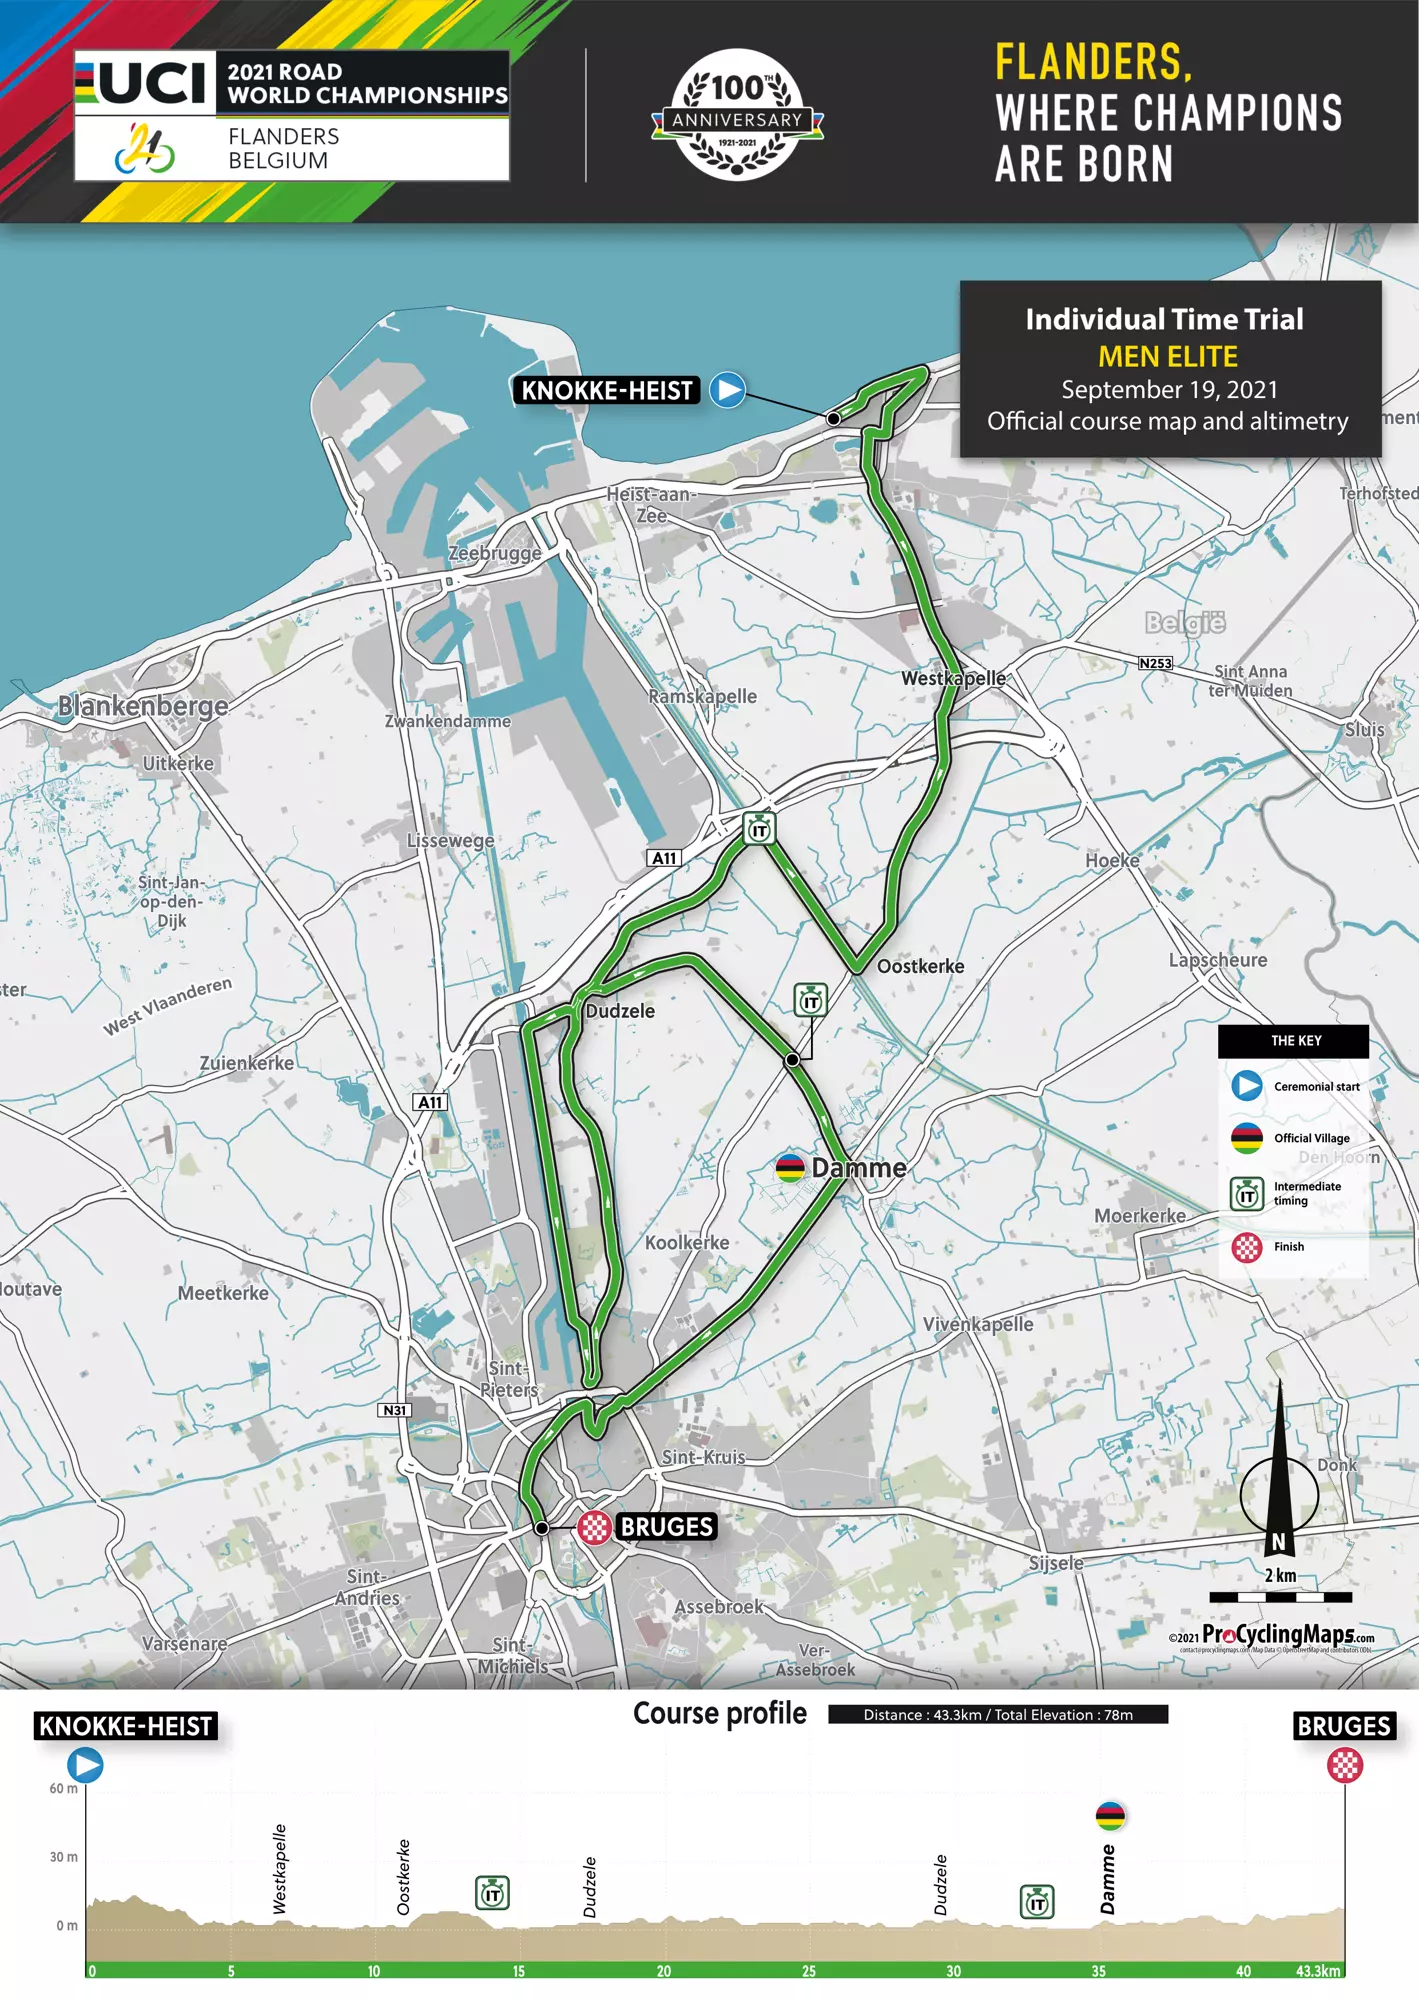
\includegraphics[width=1\columnwidth]{men-elite-individual-time-tria-map}
    \caption{course profile(from https://www.flanders2021.com)}
\end{figure}

\begin{figure}
    \centering
    \includegraphics[scale=1]{figure/men_elite_map}
    \caption{men elite map}
    \label{figure}
\end{figure}

\section{Requirement 3}
Now we take the influence of the wind into account, we will take $v_m$, which means the speed of wind, into account to simulate the influence of the weather.
\section{Requirement4}


\section{Requirement 5}


\newpage
\section{Requirement 6}
\begin{center}
    \huge \textbf{Rider's Guidance}
\end{center}\large
You have been training and focussing on this race for a while; you  have just progressed from youth races to your first junior race; you are experienced in riding.
However, taking part in the race on the open road in a bunch is an exciting challenge, and you don't want to make any mistakes.
Understanding the techniques, skills, etiquette and rules will help keep the race safe and enjoyable for everyone. Now I must ask all of you to pay close attention to the instructions in the guide and use your power meter
to help you control your pace to meet its required so that you can make the best of yourself without hurting yourself with the high tensity of the race and your eager for
the champion. This knowledge can also significantly improve your chances of finishing in the best possible place in the results!

Time trials are called the 'race of truth' for good reason. There's no hiding in the bunch before the sprint, you have to work for your speed every inch of the way, so it
became extremely  important to keep a reasonable pace, and this guidance aims to help you do so.
Recently a new model has been developed to find the best racing strategy for each rider, from your trainings and races in the past, it was able to quantificat your ability
like stamina, recovery, critical power and maximum power the model will show you when to slow down and when to speed up, with a proper pace you will be able to ride
fast and easy.

A pre-performance routine means your attention stays in the present and only on elements that are task-relevant. It helps reduce anxiety, gets you to your optimal level
of nerves, and improves concentration, focus and performance.

The routine gets you ready to compete, feeling comfortable you have done everything possible to reach the start line with the best preparation. The more you repeat and
practice the routine, the more beneficial it is. I hope you have all remembered the instructions above, and it is ok if you didn't, you will remember them in a few routines.
Now go!
%%%%%%%%%%%%%%%%%%%%%%%%%%%%%%
\bibliographystyle{plain}
\bibliography{2022_MCM_ICM_Report}
\end{document}
\end
